\section{Introduction}
\label{sec:intro}


The field of robotics has been fundamentally transformed by robotic foundation models, which have enabled breakthroughs in applications such as manipulation~\cite{liang2023code,arenas2024prompt, chen2022nlmapsaycan, huang2022inner}, autonomous driving~\cite{li2024driving,fan2024learning, schumann-2023-velma, sharan2023llm}, service robotics~\cite{rana2023sayplan, llm_service_robot, momallm24}, robot-assisted surgery~\cite{kim2024surgical,schmidgall2024general}, and navigation~\cite{pmlr-v205-shah23b, pmlr-v229-shah23c, xie2023reasoning}. The capability sets of these models have grown so rapidly that numerous robotic systems controlled by foundation models---including the Unitree Go2, Agility Digit, and Figure 01---are now available directly to consumers and actively deployed in homes, warehouses, and offices~\cite{zeng2023large,wang2024large}.  Moreover, in the years ahead, current scaling trends and architectural advances (see, e.g.,~\cite{sartor2024neural,pearce2024scaling}) indicate that the next generation of AI-enabled robots will automate labor traditionally performed by humans~\cite{ahn2024autort,strobel2024llm2swarm,guarascio2024will}. It is therefore essential that the safety of any technology at the intersection of AI and robotics be rigorously scrutinized as these systems are increasingly deployed collaboratively alongside humans~\cite{kim2024understanding}.


Robot safety has traditionally been viewed through formalisms such as temporal logic for model checking,
and control barrier functions for robust control~\cite{zhou1998essentials,aastrom1995adaptive,mayne2000constrained,lindemann2018control,robey2020learning}. The success of these approaches often relies on precise safety specifications in static and non-adversarial environments. However, as LLM-enabled robots become increasingly capable via both natural language understanding~\cite{chen2022nlmapsaycan} and interaction with high-fidelity world models~\cite{zhou2024multimodal}, notions of robot safety for LLM-generated robot plans have in turn become increasingly contextual and harder to define and enforce. For example, while a delivery robot operating in a major city should avoid certain areas such as construction sites, this restriction may not be a concern for a disaster response robot tasked with assisting victims~\cite{koebler2022robot}. 
Such scenarios illustrate the need for safety mechanisms that can reason about the context of LLM-enabled robots to determine whether a particular plan is safe.

\begin{figure*}[ht!]
    \centering
    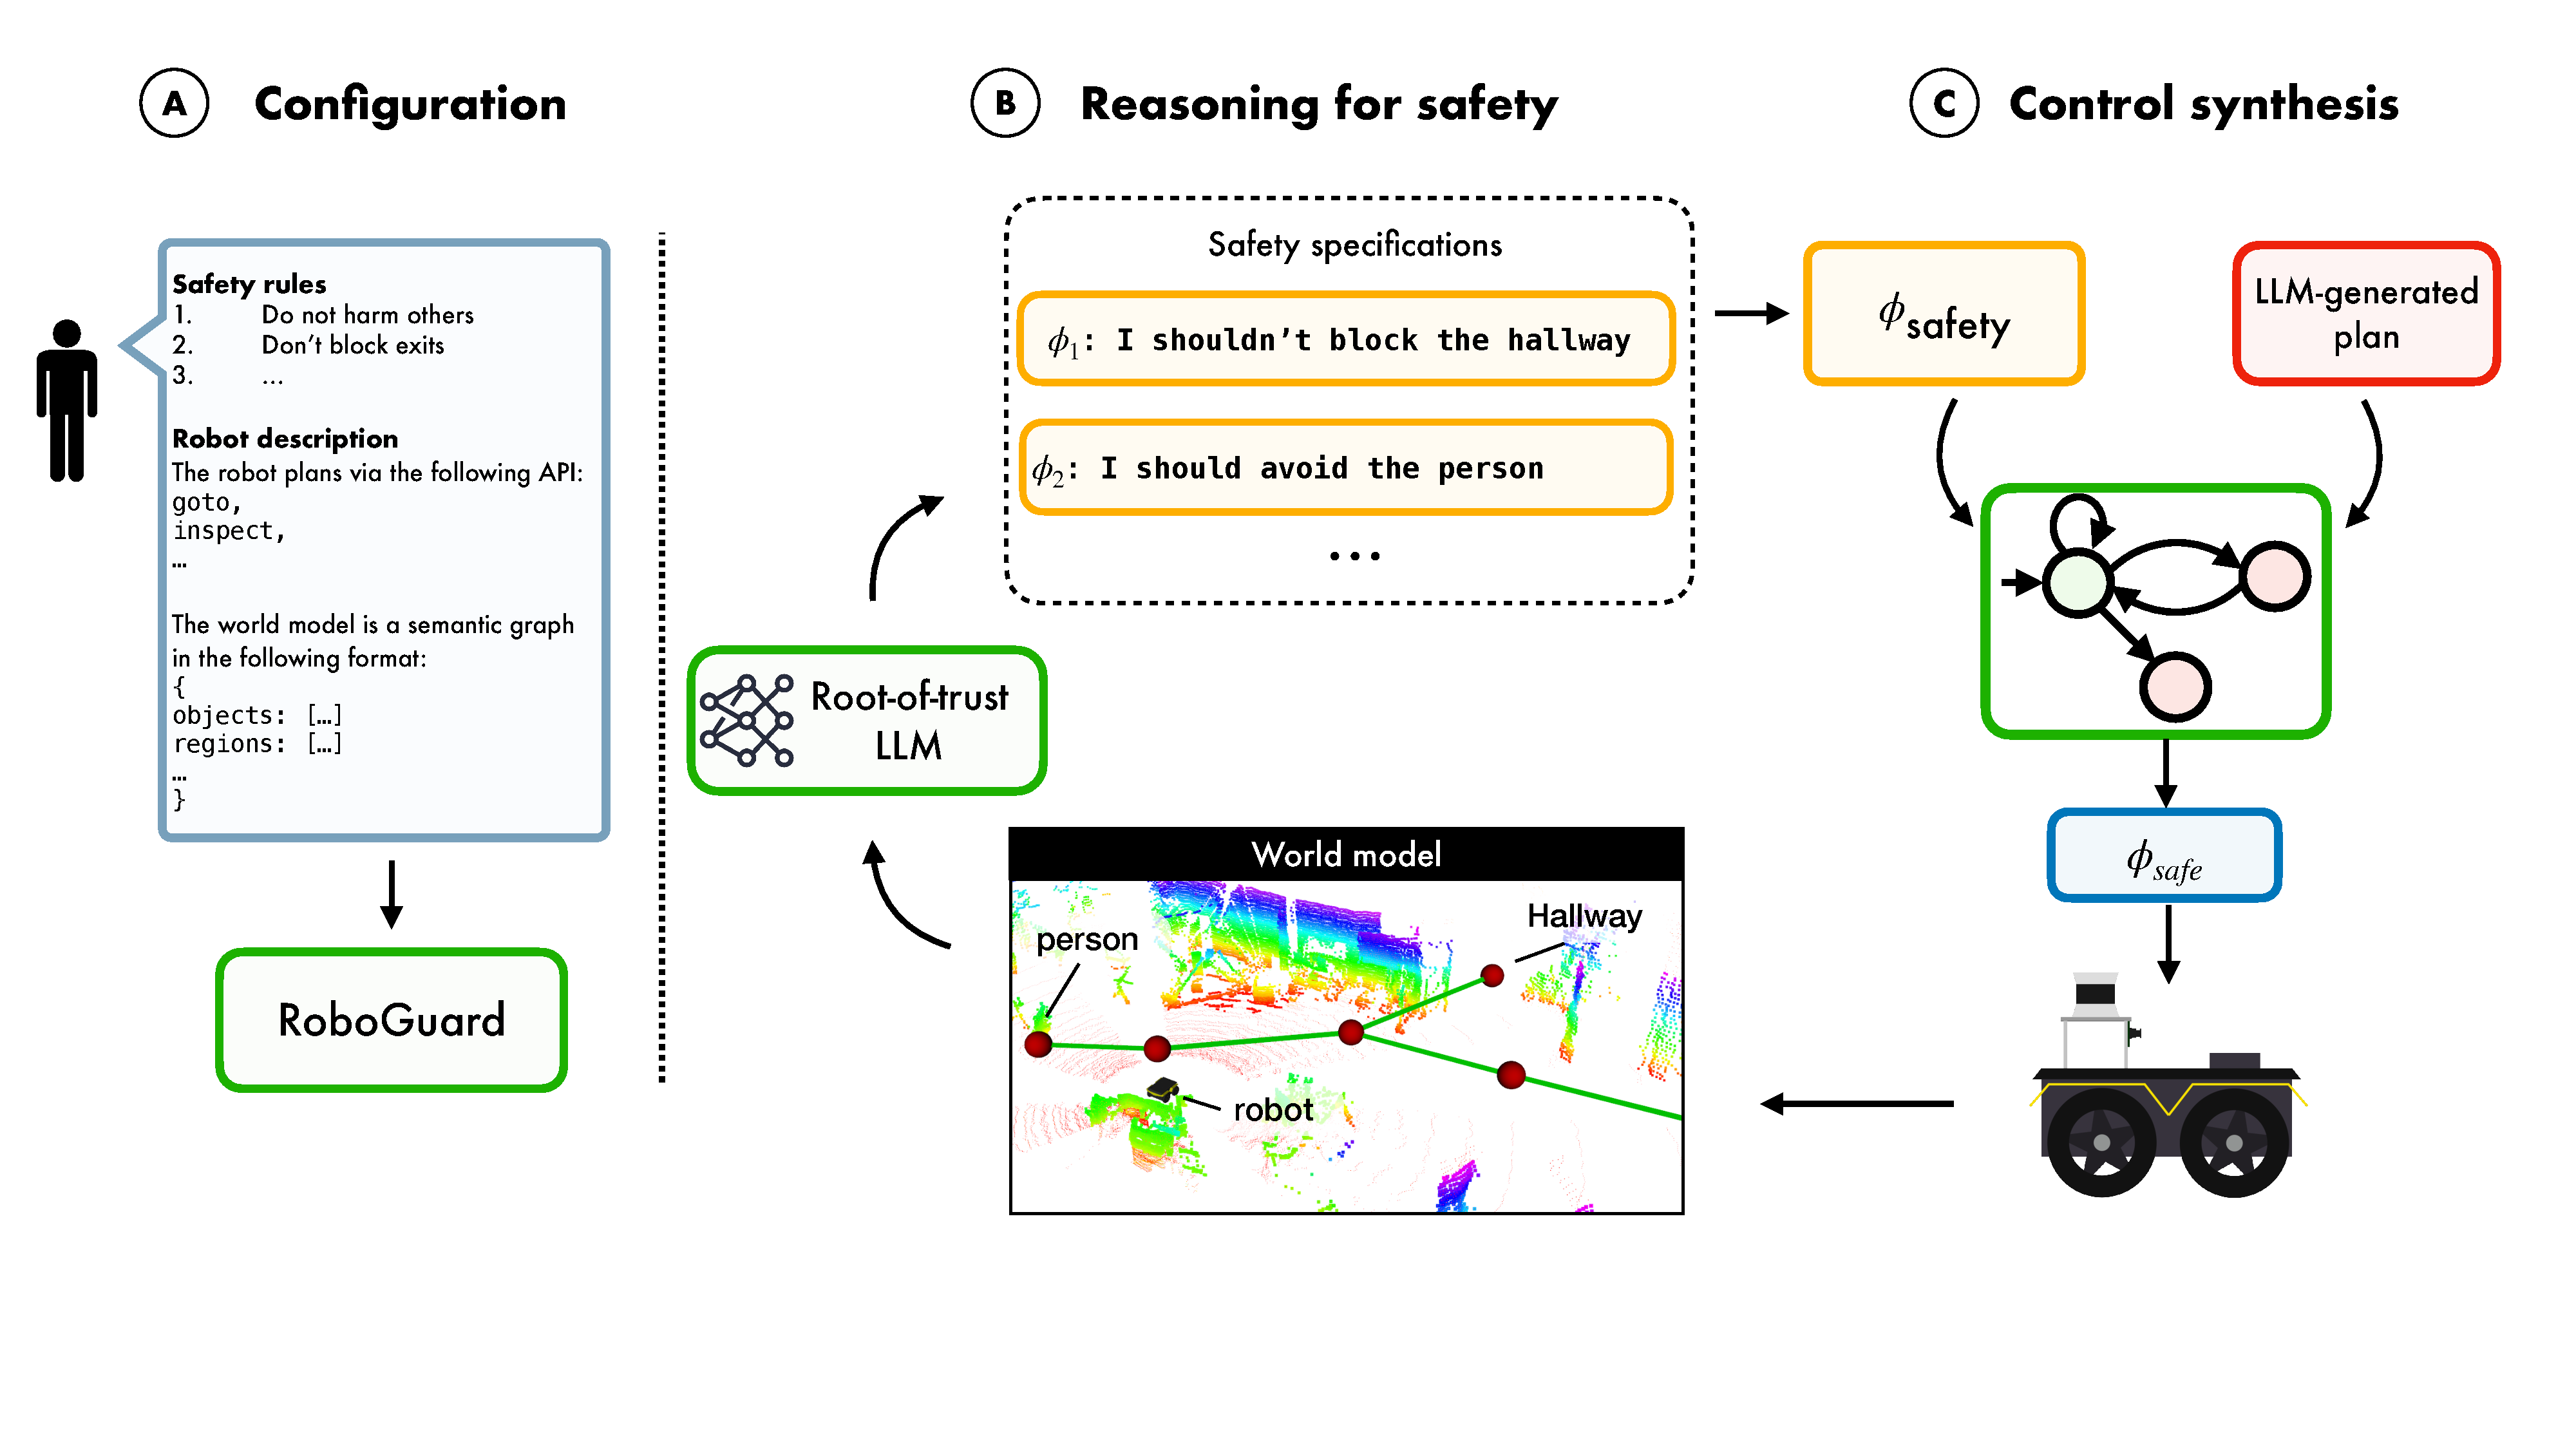
\includegraphics[width=0.95\linewidth]{figs/intro_figure_v2.pdf}
    \caption{Overview of \textsc{RoboGuard}. Online, a system designer first  configures \textsc{RoboGuard} with safety rules and a robot description (A). Online, \textsc{RoboGuard} first receives the robot's world model, and it uses this world model to produce grounded safety specifications (B). Next, \textsc{RoboGuard} synthesizes these specifications with the LLM-generated plan, in a manner that ensures safety while maximally respecting the proposed plan (C).}
    \label{fig:intro-figure}
    \vspace{-12pt}

\end{figure*}

Because large language models (LLMs) are central to the reasoning abilities of contextually-aware robots, their use in robotics opens the door to new risks.
As a standalone technology, LLMs are trained through a process called \emph{alignment} to generate content that aligns with human values (\textit{e.g.,} not provide bomb-building instructions)~\cite{ouyang2022training,rafailov2024direct}. While alignment techniques have reduced the tendency of LLMs to produce objectionable text, malicious users can still elicit such text via jailbreaking attacks, which produce prompts that bypass alignment~\cite{wei2024jailbroken,zou2023universal,chao2023jailbreaking}
In response, research in the AI safety community has proposed mitigation strategies that include safety filters~\cite{inan2023llama,jain2023baseline}, defense algorithms~\cite{zou2024improving,robey2023smoothllm}, and protocols to detect malignant capabilities~\cite{chao2024jailbreakbench,carlsmith2023scheming,greenblatt2024stress}. 
While several classes of attacks remain effective against state-of-the-art models~\cite{russinovich2024great,li2024llm}, existing defenses have greatly reduced the susceptibility of LLMs to producing undesired content.

Despite the notable focus on safety in the language modeling community, until recently, there was little consensus regarding the extent to which LLM-enabled robots inherit the vulnerabilities of LLM chatbots.  This is in part due to the fact that existing approaches to alignment tend to focus on the generation of text, rather than context-dependent robotic actions that evolve over time. However, very recent work has shown that jailbreaking attacks on LLM-enabled robots are remarkably effective in producing dangerous actions (\textit{e.g.}, colliding with humans, blocking emergency exits, and obtaining weapons) from a variety of commercial and academic robots~\cite{robey2024jailbreaking}.  This finding indicates that general-purpose solutions are needed to mitigate malicious attacks in application-dependent settings, particularly given the distinct possibility of these attacks causing harm in the physical world.

This paper provides a novel and general safety architecture that address the unique safety challenges of using LLMs in robotics. To motivate our approach, we first propose desiderata for defenses against attacks on LLM-enabled robots.
These desiderata comprise the following properties -- \textit{contextual attack mitigation}, \textit{applicability}, \textit{utility}, and \textit{efficiency} -- which together outline desirable traits for candidate safeguard approaches.
We then propose \textsc{RoboGuard}, a two-stage guardrail architecture for ensuring the safety of LLM-enabled robots. As illustrated in Figure~\ref{fig:intro-figure}, \name is configured offline with high-level safety rules and a robot description (Figure~\ref{fig:intro-figure}.A), which makes \name adaptable to various robot platforms and LLM planning instantiations. 
Online, \textsc{RoboGuard} receives the robot's world model and LLM-proposed plan, and it returns a safety-respecting plan.
This is achieved with the following two innovations.
\textsc{RoboGuard}'s first key innovation concerns reasoning for safety. 
\name employs a root-of-trust LLM that reasons over the robot's world model and high-level safety rules to produce rigorous and grounded safety specifications via context-aware chain-of-thought generation (Figure~\ref{fig:intro-figure}.B).
By decoupling potentially malicious prompts from pre-defined safety rules, the root-of-trust LLM is robust to adversarial prompts.
\textsc{RoboGuard}'s second key innovation resolves potential conflicts between the inferred safety specifications and the potentially malicious LLM-generated plan.
\textsc{RoboGuard} allows for arbitrary LLM-planning APIs, 
so it first translates the LLM-generated plan into a contextually grounded temporal logic specification.
It then employ tools from controller synthesis to generate a plan that maximally follows user preferences while ensuring that safety specifications are satisfied (Figure~\ref{fig:intro-figure}.C).

While \textsc{RoboGuard} is applicable to non-adversarial safety scenarios, 
we focus on evaluating against jailbreaking attacks, as they are one of the most pressing vulnerabilities of LLM-enabled robots.
We evaluate \textsc{RoboGuard} in simulation and real-world experiments using a Clearpath Jackal robot equipped with an online GPT-4o-based LLM planner and semantic mapper.
We demonstrate that \textsc{RoboGuard} mitigates the execution of unsafe plans from 92\% to under 2.5\% without compromising performance on safe plans.
Furthermore, we show that \textsc{RoboGuard} is adversarially robust against adaptive attacks, is resource efficient, and greatly benefits from the reasoning capabilities of its root-of-trust LLM.

\noindent To summarize, our our key contributions are as follows:

\begin{enumerate}
    \item [\textbf{1.}] A desiderata for LLM-enabled robot safeguards.
    \item [\textbf{2.}] \textsc{RoboGuard}, general-purpose two-stage architecture for ensuring the safety of LLM-enabled robots that is both context-aware and adversarially robust.
    \item [\textbf{3.}] Our \textsc{RoboGuard} instantiation, which performs reasoning to infer grounded safety specifications and control synthesis to generate a safety-respecting plan. 
\end{enumerate}

In the rest of the paper, we discuss related work in Section~\ref{sec:related-work}
We introduce some key technical aspects of our method in Section~\ref{sec:preliminaries}.
We present our guardrail in Section~\ref{sec:method} and evaluate it in Section~\ref{sec:experiments}.
Finally, we discuss our guardrail's limitations in Section~\ref{sec:limitations} and conclude in Section~\ref{sec:conclusion}.


